\section{Kitting Problem}
\label{S:kitting-problem}
The kitting problem is quite complex and contains far too many states to represent them all explicitly. Using an example of kit to build, this section will only describe the initial and goal states explicitly. The operators detailed in Section~\ref{subsect:Planning_Operators} are used by a planner to generate the other states as needed.\\
In this example, the \class{Robot} has to build a kit that contains two \class{Parts} of type A, two \class{Part} of type B and one \class{Part} of type C. The kitting process is completed once the kit is placed in the \class{LargeBoxWithKits}.

\paragraph{Constant Variable Symbols}
Constant variable symbols for the kitting domain are part of the PDDL problem file and are presented in Figure~\ref{fig:objects}.
\begin{figure}[t!h!]
\centering
\begin{minipage}{.5\paperwidth}
\begin{mylisting}
\begin{Verbatim}[commandchars=\\\{\},fontsize=\scriptsize, numbers=left, numbersep=2pt]
(:objects
    robot_1 - Robot
    changing_station_1 - EndEffectorChangingStation
    kit_tray_1 - KitTray
    kit_a2b2c1 - Kit
    empty_kit_tray_supply - LargeBoxWithEmptyKitTrays
    finished_kit_receiver - LargeBoxWithKits
    work_table_1 - WorkTable
    part_a_tray part_b_tray part_c_tray - PartsTray
    part_a_1 part_a_2 part_a_3 part_a_4 - Part
    part_b_1 part_b_2 part_b_3 part_b_4 - Part
    part_c_1 part_c_2 part_c_3 part_c_4 - Part
    part_gripper tray_gripper - EndEffector
    part_gripper_holder tray_gripper_holder - EndEffectorHolder
)
\end{Verbatim}
\end{mylisting}
\end{minipage}
\caption{Representation of constant variable symbols in PDDL.}
\label{fig:objects}
\end{figure}

\texttt{objects} signals a planner that the constant variable symbols from line 2 to line 14 are available in the kitting workstation.





\subsection{Initial State}
The initial state $s_0$ (Figure~\ref{fig:s0}) defines the predicates that are true in the kitting workstation. The initial state of the kitting problem is described in Figure~\ref{fig:init}. Some relevant parts of the init section are described further in this section.

\begin{figure}[h!b!]
\centering
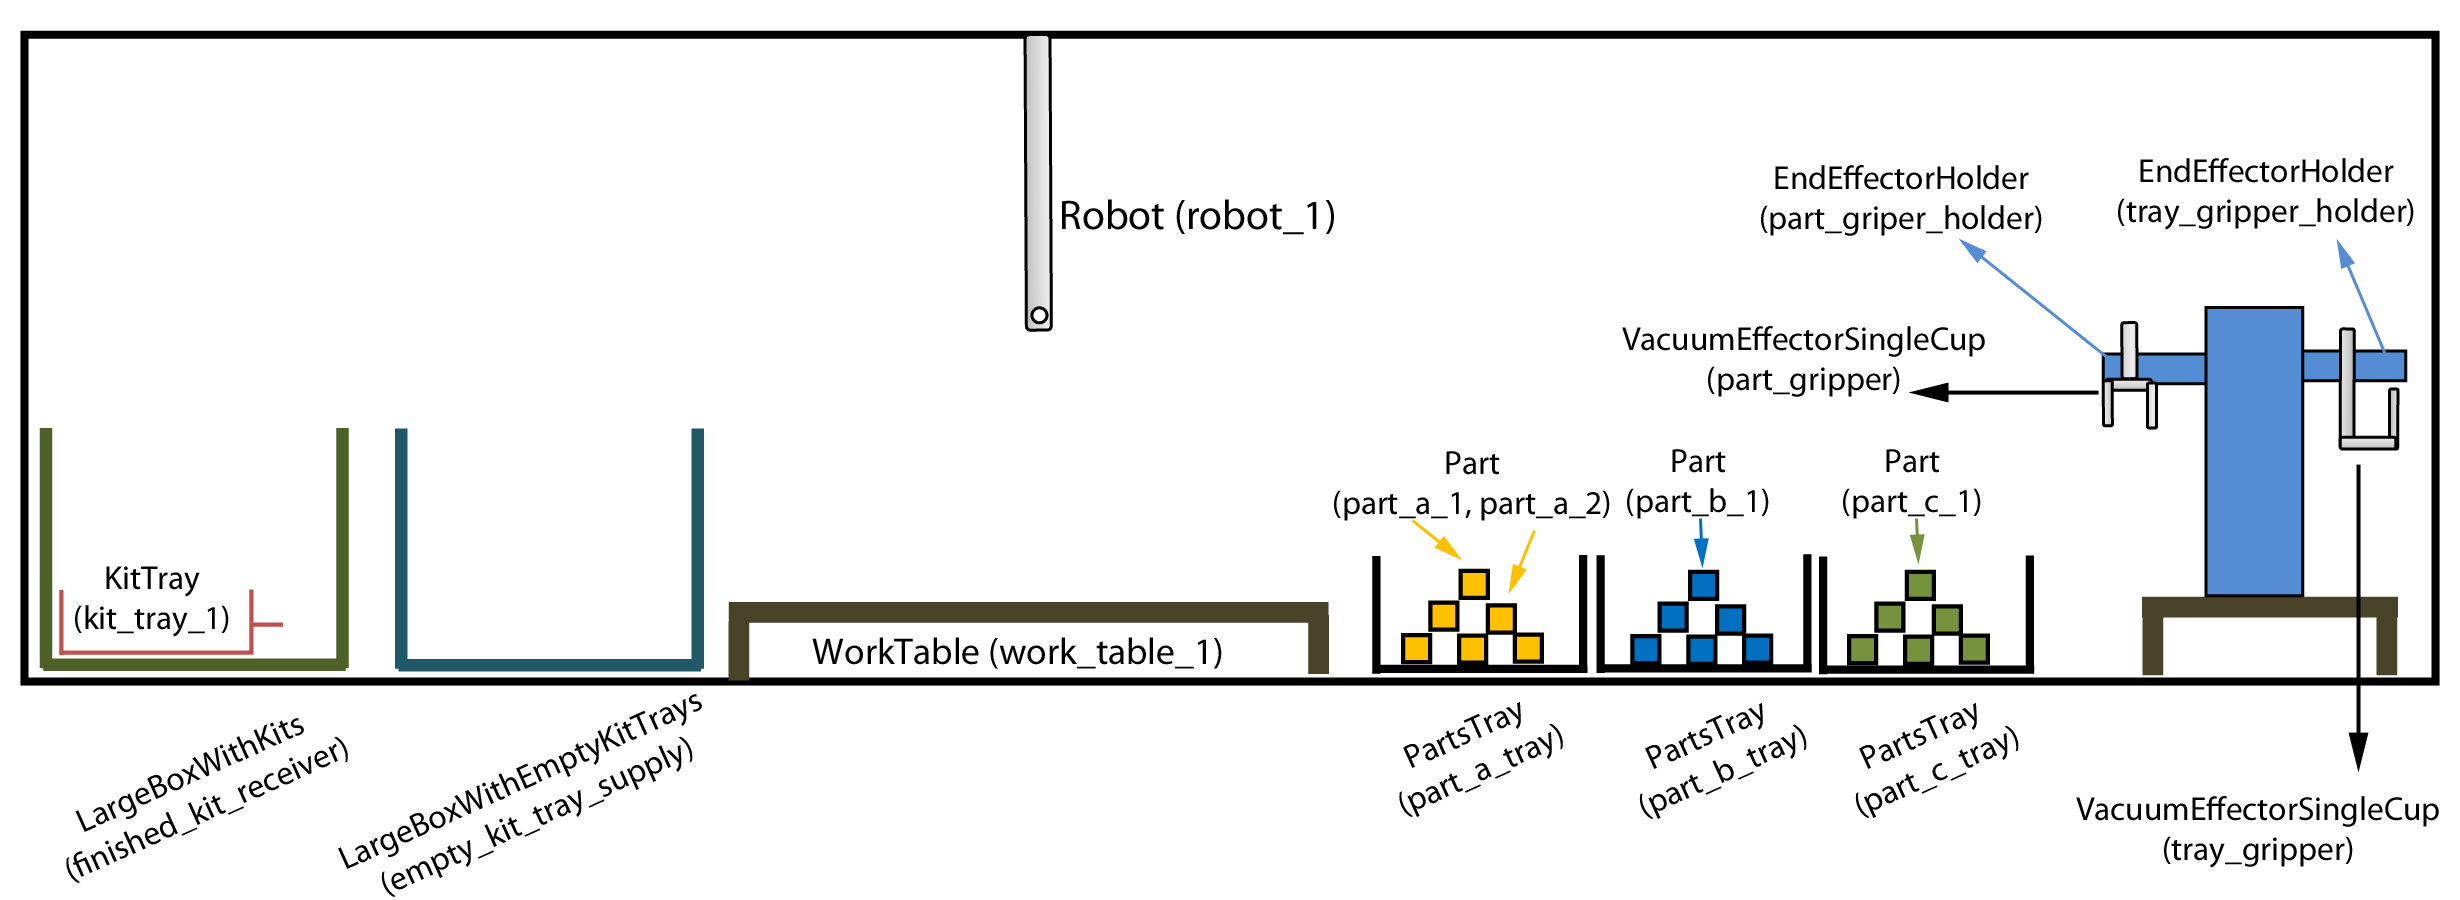
\includegraphics[width=16cm]{Figure/s0.jpg}
\caption{Initial state.}
\label{fig:s0}
\end{figure}

\begin{figure}[t!h!]
\centering
\begin{minipage}{.5\paperwidth}
\begin{mylisting}
\begin{Verbatim}[commandchars=\\\{\},fontsize=\scriptsize, numbers=left, numbersep=2pt]
(:init
    (robot-with-no-endeffector robot_1)
    (part-not-searched)
    (lbwekt-not-empty empty_kit_tray_supply)	
    (lbwk-not-full finished_kit_receiver)		
    (partstray-not-empty part_a_tray)
    (partstray-not-empty part_b_tray)
    (partstray-not-empty part_c_tray)
    (endeffector-location-endeffectorholder part_gripper part_gripper_holder)
    (endeffector-location-endeffectorholder tray_gripper tray_gripper_holder)
    (endeffectorholder-holds-endeffector part_gripper_holder part_gripper)
    (endeffectorholder-holds-endeffector tray_gripper_holder tray_gripper)
    (endeffectorholder-location tray_gripper_holder changing_station_1)
    (endeffectorholder-location part_gripper_holder changing_station_1)
    (endeffectorchangingstation-contains-endeffectorholder changing_station_1 tray_gripper_holder)	
    (endeffectorchangingstation-contains-endeffectorholder changing_station_1 part_gripper_holder)
    (worktable-empty work_table_1)
    (kittray-location-lbwekt kit_tray_1 empty_kit_tray_supply)
\end{Verbatim}
\end{mylisting}
\end{minipage}
	
\begin{minipage}{.5\paperwidth}
\begin{mylisting}
\begin{Verbatim}[commandchars=\\\{\},fontsize=\scriptsize,  firstnumber=continue, numbers=left, numbersep=2pt]	
    (part-location-partstray part_a_1 part_a_tray)
    (part-location-partstray part_a_2 part_a_tray)
    (part-location-partstray part_a_3 part_a_tray)
    (part-location-partstray part_a_4 part_a_tray)
    (part-location-partstray part_b_1 part_b_tray)
    (part-location-partstray part_b_2 part_b_tray)
    (part-location-partstray part_b_3 part_b_tray)
    (part-location-partstray part_b_4 part_b_tray)
    (part-location-partstray part_c_1 part_c_tray)
    (part-location-partstray part_c_2 part_c_tray)
    (part-location-partstray part_c_3 part_c_tray)
    (part-location-partstray part_c_4 part_c_tray)
\end{Verbatim}
\end{mylisting}
\end{minipage}
	
\begin{minipage}{.5\paperwidth}
\begin{mylisting}
\begin{Verbatim}[commandchars=\\\{\},fontsize=\scriptsize,  firstnumber=continue, numbers=left, numbersep=2pt]	
    (endeffector-type-part part_gripper part_a_1)
    (endeffector-type-part part_gripper part_a_2)
    (endeffector-type-part part_gripper part_a_3)
    (endeffector-type-part part_gripper part_a_4)
    (endeffector-type-part part_gripper part_b_1)
    (endeffector-type-part part_gripper part_b_2)
    (endeffector-type-part part_gripper part_b_3)
    (endeffector-type-part part_gripper part_b_4)
    (endeffector-type-part part_gripper part_c_1)
    (endeffector-type-part part_gripper part_c_2)
    (endeffector-type-part part_gripper part_c_3)
    (endeffector-type-part part_gripper part_c_4)
    (endeffector-type-kittray tray_gripper kit_tray_1)
    (endeffector-type-kit tray_gripper kit_a2b2c1)
\end{Verbatim}
\end{mylisting}
\end{minipage}
	
\begin{minipage}{.5\paperwidth}
\begin{mylisting}
\begin{Verbatim}[commandchars=\\\{\},fontsize=\scriptsize,  firstnumber=continue, numbers=left, numbersep=2pt]	
    (= (capacity-kit kit_a2b2c1 part_a_tray) 2)
    (= (capacity-kit kit_a2b2c1 part_b_tray) 2)
    (= (capacity-kit kit_a2b2c1 part_c_tray) 1)
    (= (quantity-kit kit_a2b2c1 part_a_tray) 0)
    (= (quantity-kit kit_a2b2c1 part_b_tray) 0)
    (= (quantity-kit kit_a2b2c1 part_c_tray) 0)
    (= (quantity-partstray part_a_tray) 4)
    (= (quantity-partstray part_b_tray) 4)
    (= (quantity-partstray part_c_tray) 4)
\end{Verbatim}
\end{mylisting}
\end{minipage}
\begin{minipage}{.5\paperwidth}
\begin{mylisting}
\begin{Verbatim}[commandchars=\\\{\},fontsize=\scriptsize,  firstnumber=continue, numbers=left, numbersep=2pt]	
    (origin-part part_a_2 part_a_tray)
    (origin-part part_a_3 part_a_tray)
    (origin-part part_a_4 part_a_tray)
    (origin-part part_a_1 part_a_tray)
    (origin-part part_b_1 part_b_tray)
    (origin-part part_b_2 part_b_tray)
    (origin-part part_b_3 part_b_tray)
    (origin-part part_b_4 part_b_tray)
    (origin-part part_c_1 part_c_tray)
    (origin-part part_c_2 part_c_tray)
    (origin-part part_c_3 part_c_tray)
    (origin-part part_c_4 part_c_tray)
)
\end{Verbatim}
\end{mylisting}
\end{minipage}
\caption{The init section.}
\label{fig:init}
\end{figure}





\newpage
\subsection{Goal State}

The goal state $s_G$ (Figure~\ref{fig:sf}) defines the predicates that are true in the final state. In the goal state, \class{Parts} \const{part\_a\_1}, \const{part\_a\_2}, \const{part\_b\_1}, and \const{part\_c\_1} are in the \class{Kit} \const{kit\_1}. \const{kit\_1} is placed in the \class{LargeBoxWithKits} \const{finished\_kit\_receiver}. $s_G$ is represented in Table~\ref{table:final}.

\begin{table}[h!t!p!]
\caption{Final State $s_G$}
\centering
\begin{tabular}{|l|l|}
  \hline
  \hline
  \stvar{part-location}(\const{part\_a\_1},\const{kit\_1})\\
  \stvar{part-location}(\const{part\_a\_2},\const{kit\_1})\\
  \stvar{part-location}(\const{part\_b\_1},\const{kit\_1})\\
  \stvar{part-location}(\const{part\_c\_1},\const{kit\_1})\\
  \stvar{kit-location}(\const{kit\_1},\const{finished\_kit\_receiver})\\
  \hline
\end{tabular}
\label{table:final}
\end{table}
\begin{figure}[h!t!]
\centering
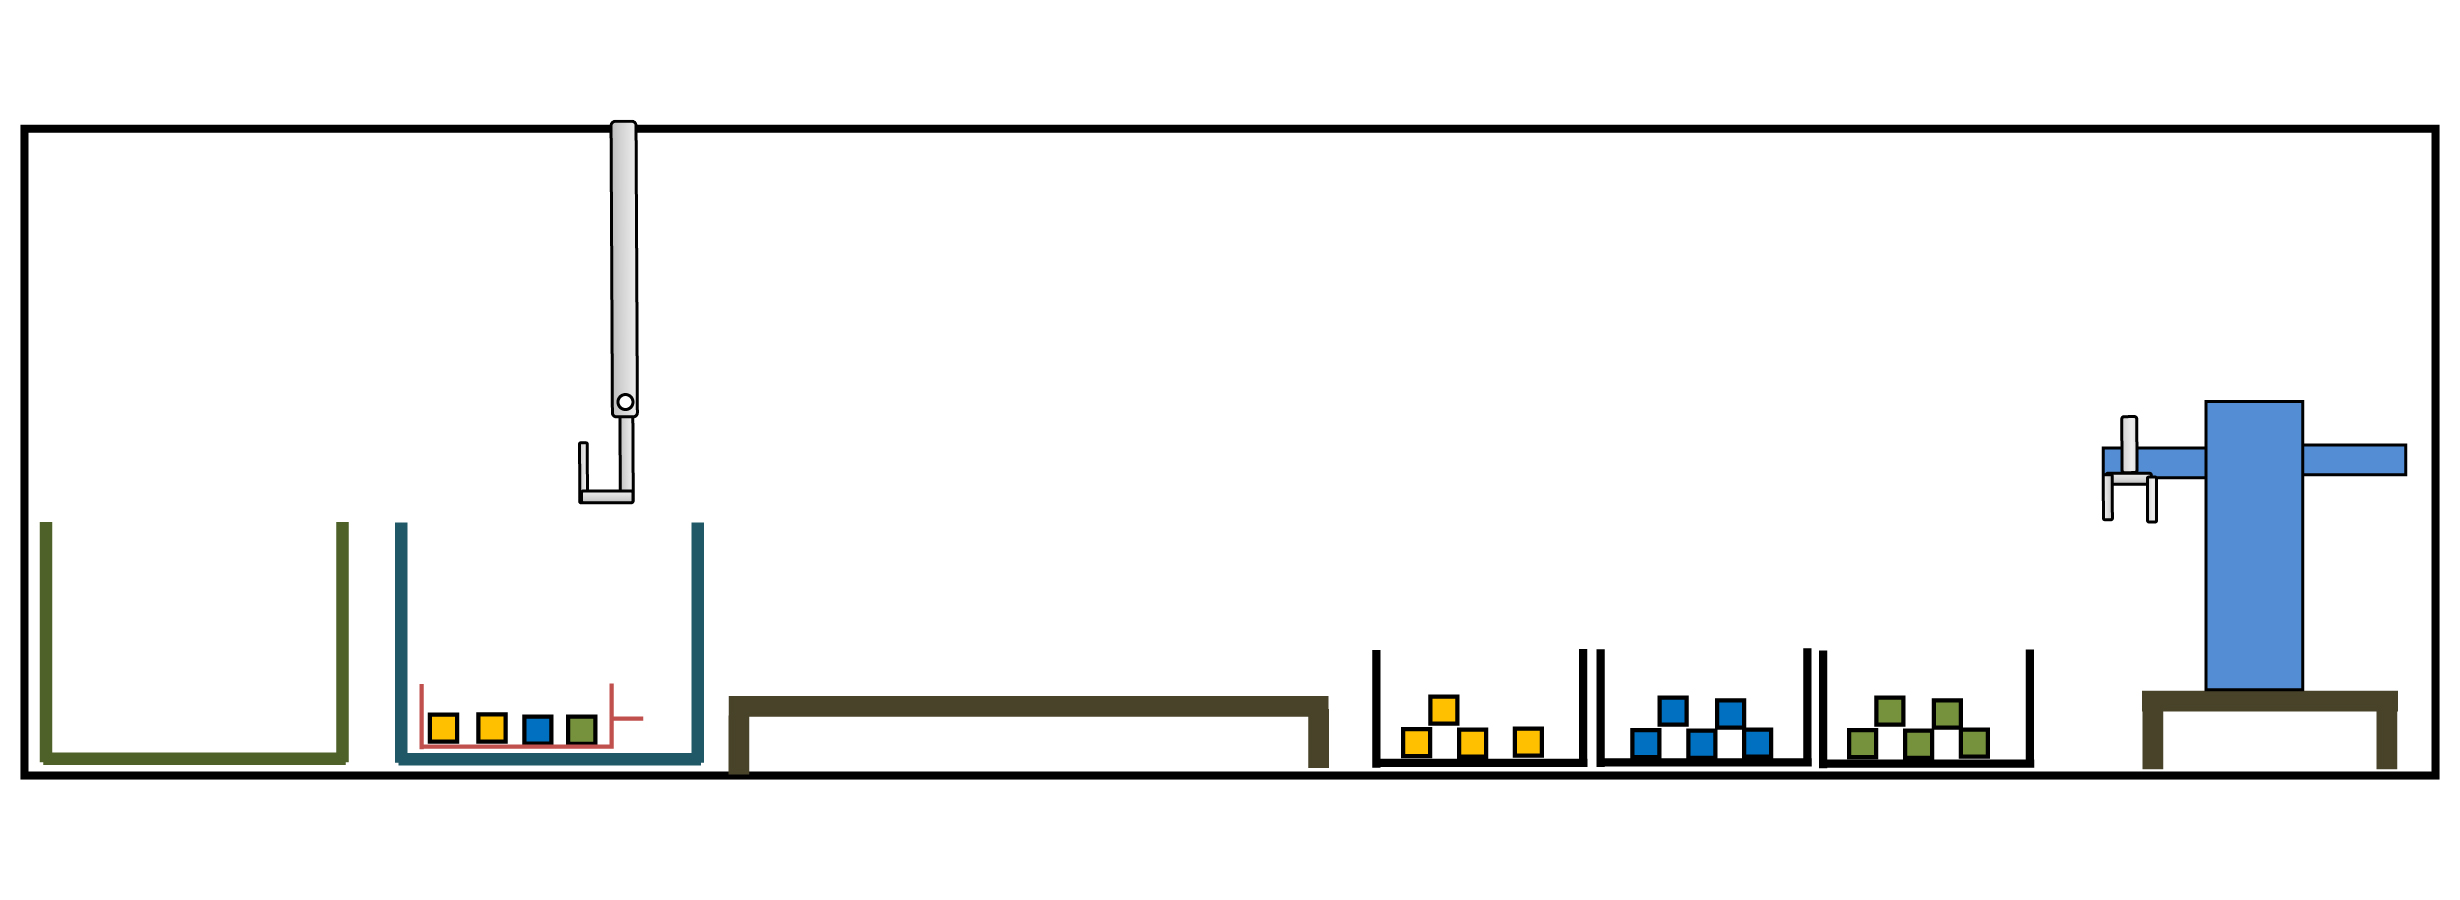
\includegraphics[width=16cm]{Figure/sfinal.jpg}
\caption{Goal state.}
\label{fig:sf}
\end{figure} 

